\chapter{The Method of Characteristics}
\label{chap:moc}

Standard \ac{MOC} solvers, such as the one developed and discussed in this thesis, solve the multi-group transport equations, relying on multi-group cross-sections, allowing the computation of reaction rates across any reactor geometry. This chapter discusses the \ac{MOC} method, including both theoretical and practical aspects.

First, the multi-group transport equation is discussed. Then, the \ac{MOC} equations are derived from the multi-group transport equation for both flat and linear source approximations. This chapter highlights the important equations for an \ac{MOC} implementation and algorithmic considerations are noted.

%First, the multi-group transport equation is discussed in Section~\ref{sec:multi-group-transport}. Then, the \ac{MOC} equations are derived from the multi-group neutron transport equation in Section~\ref{sec:derivation-of-moc}. Track discretization is introduced in Section~\ref{sec:track-disceretization}, forming a system of equations involving discrete variables. Simplifications from the track laydown are discussed in Section~\ref{sec:track-simplifications}, with a concentration on the volume calculation. The flat source approximation is discussed in Section~\ref{sec:flat-source}. In Section~\ref{sec:linear-source}, the 2D track-based linear source approximation developed by Ferrer~\cite{ferrer2015linear} is expanded to three dimensions. In Section~\ref{sec:ls-algorithm}, algorithmic aspects of the linear source approximation are discussed.

%Discussions of solution techniques to the \ac{MOC} system of equations are normally centered around the underlying physics with little mention of the system as a linear algebra problem~\cite{boyd2014openmoc}. Others further describe \ac{MOC} in terms of operator notation~\cite{mocfe_init, kochunas}, but these discussions often offer little insight into the structure of the operators. Instead, this discussion casts the system of equations as simply a general eigenvalue problem. Discussion of matrix structure motivates the use of \textit{source iteration}. Physical reasoning for the structure is mentioned throughout the discussion. The properties of \textit{source iteration} are discussed, motivating the need for an acceleration scheme to mitigate its weaknesses.


%%%%%%%%%%%%%%%%%%%%%%%%%%%%%%%%%%%%%%%%%%%%%%%%%%%%%%%%%%%%%%%%%%%%%%%%%%%%%%%
\section{The Multi-Group Transport Equation}
\label{sec:multi-group-transport}

The ultimate goal in neutron transport analysis is to determine the rates of neutron-induced reactions throughout the reactor core. Neutrons can undergo various reactions when they strike materials of the reactor core, often referred to as \textit{target nuclei}. These interactions include scattering, capture, and fission, though others exist as well, and understanding neutron behavior is critical to determining the reaction rates.

The neutron population can be categorized by location $\mathbf{r}$, direction of travel $\mathbf{\Omega}$, and energy. In this thesis, multi-group transport is studied in which the continuous energy variable has been discretized into a number of energy groups. Reaction rates $R_X^g$ of type $X$ in energy group $g$ can be calculated with multi-group cross-sections $\Sigma_X^g$ and the \textit{neutron angular flux} $\psi_{g}$ as
\begin{equation}
R_X^g(\mathbf{r}, \mathbf{\Omega}) = \Sigma_X^g(\mathbf{r}, \mathbf{\Omega}) \psi_{g}(\mathbf{r},\mathbf{\Omega})
\end{equation}
where the neutron angular flux $\psi_{g}$ characterizes neutrons along a certain direction.  Often, the cross-sections are independent of angle and integrated reaction rates over all angles are desired. This motivates the determination of \textit{neutron scalar fluxes} $\phi_g(\mathbf{r})$, defined by
\begin{equation}
\phi_{g}(\mathbf{r}) = \int_{4\pi} d\mathbf{\Omega} \, \psi_{g}(\mathbf{r},\mathbf{\Omega}),
\label{eqn:scalar-flux}
\end{equation}
to often be the goal of neutron simulations. Cross-sections have a continuous energy dependence but reaction rates can be preserved with multi-group cross-sections through the use of the scalar flux. Specifically, the multi-group cross-sections $\Sigma_X^g$ for group $g$ with energy bounds $E_g$ and $E_{g-1}$ are formed using the continuous-energy scalar flux $\phi$ as
\begin{equation}
\Sigma_{X}^g(\mathbf{r}) = \frac{\int_{E_{g}}^{E_{g-1}} dE \, \Sigma_{X}(\mathbf{r},E)\phi(\mathbf{r},E)}{\int_{E_{g}}^{E_{g-1}} dE \, \phi(\mathbf{r},E)}.
\label{eqn:mgxs}
\end{equation}
It is important to note that the scalar flux is the solution of neutron transport simulation. Therefore, the correct scalar flux solution is necessary in order to form accurate cross-sections. Since such knowledge is not practical, approximations of the neutron flux are used to form multi-group cross-sections\cite{boyd2017thesis}. A depiction of this process is shown in Figure~\ref{fig:microscopic-to-multigroup}.
\begin{figure}[h!]
	\centering
	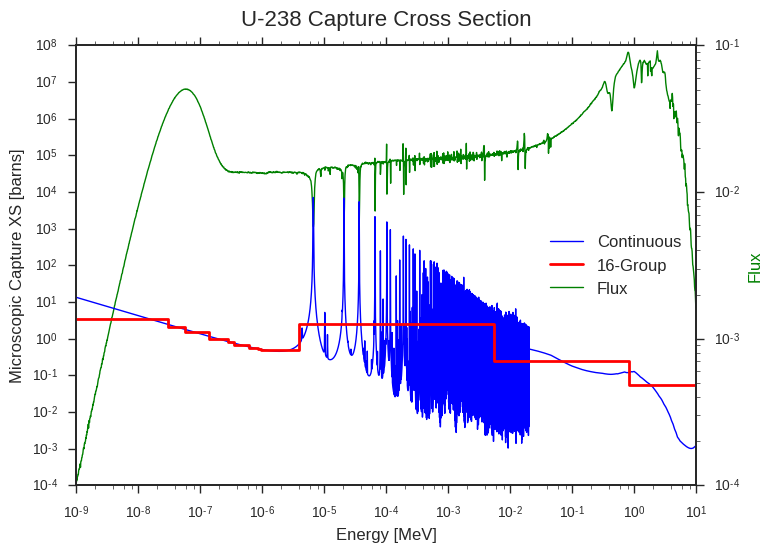
\includegraphics[width=0.9\linewidth]{figures/u238-capture-16.png}
	\caption[]{An illustration of forming multi-group cross-sections from continuous energy cross-sections showing the continuous energy capture cross-section of U-238 (blue), the neutron flux (green), and the multi-group representation with 16 groups (red).}
	\label{fig:microscopic-to-multigroup}
\end{figure}
Once multi-group cross-sections are formed, a balance of neutron losses and gains can yield the steady-state neutron transport equations. The relevant losses are net neutron leakage and total reaction rate with materials. The relevant neutron gains are neutron production from fission and in-scattering from other energy groups. This leads to the neutron transport equation\cite{henry, duderstadt, duderstadt-martin, bell1967transport, hebert2009applied} which describes the balance of loss and source terms in Eq.~\ref{eqn:multi-group-transport}.
\begin{equation}
\begin{split}
\mathbf{\Omega} \cdot \nabla \psi_{g}(\mathbf{r},\mathbf{\Omega}) & \, + \, \Sigma_t^{g}(\mathbf{r},\mathbf{\Omega}) \psi_{g}(\mathbf{r},\mathbf{\Omega}) =  \\
& \frac{1}{4 \pi} \left( \frac{\chi_{g}\left(\mathbf{r}\right)}{k} \sum_{g'=1}^{G} \nu_{g'}\left(\mathbf{r}\right) \Sigma_f^{g'}\left(\mathbf{r}\right) \phi_{g'}\left(\mathbf{r}\right) + \, \sum_{g'=1}^G \,  \Sigma_{s}^{g' \rightarrow g}\left(\mathbf{r}\right) \phi_{g'}(\mathbf{r}) \right)
\end{split}
\label{eqn:multi-group-transport}
\end{equation}
where $\Sigma_t^{g}$ is the total cross-section, $\chi_{g}$ is the neutron emission spectrum, $\nu$ is the average number of neutrons released per fission, $\Sigma_f^{g}$ is the fission cross-section, $\Sigma_{s}^{g' \rightarrow g}$ is the scattering cross-section from group $g'$ to group $g$, and the total number of energy groups is $G$. The eigenvalue $k$ is applied to the fission term as one way of forcing a non-trivial solution when cross-sections are imperfectly known. If cross-sections and geometry were known to infinite precision for a steady-state system, $k$ would be exactly 1.0. The deviation of $k$ from 1.0 shows the degree to which the system is unbalanced for the supplied cross-sections.

It is important to note that the multi-group transport equation used here assumes isotropic scattering. However, neutron scattering off of light isotopes, such as hydrogen found in water, is highly anisotropic. Therefore, a \textit{transport correction}~\cite{bell1967transport} is often applied to the cross-sections to retain solution accuracy. This is discussed more thoroughly in Appendix~\ref{app:transport-correction}.


%%%%%%%%%%%%%%%%%%%%%%%%%%%%%%%%%%%%%%%%%%%%%%%%%%%%%%%%%%%%%%%%%%%%%%%%%%%%%%%
\section{Derivation of Continuous Angle MOC Equations}
\label{sec:derivation-of-moc}

Starting from the multi-group transport equation in Eq.~\ref{eqn:multi-group-transport}, the neutron source $q_g(\mathbf{r})$ can be defined by Eq.~\ref{eqn:source} as
\begin{equation}
q_g(\mathbf{r}) = \frac{1}{4 \pi} \left( \frac{\chi_{g}\left(\mathbf{r}\right)}{k} \sum_{g'=1}^{G} \nu_{g'}\left(\mathbf{r}\right) \Sigma_f^{g'}\left(\mathbf{r}\right) \phi_{g'}\left(\mathbf{r}\right) + \, \sum_{g'=1}^G \,  \Sigma_{s}^{g' \rightarrow g}\left(\mathbf{r}\right) \phi_{g'}(\mathbf{r}) \right)
\label{eqn:source}
\end{equation}
which leads to the neutron balance expression,
\begin{dmath}
	\mathbf{\Omega} \cdot \nabla \psi_g(\mathbf{r},\mathbf{\Omega}) \, + \, \Sigma_{t}^{g}(\mathbf{r})\psi_g(\mathbf{r},\mathbf{\Omega}) = q_g(\mathbf{r}).
	\label{eqn:source-balance}
\end{dmath}
Next, a coordinate transformation is performed, casting the position as a displacement from an origin $\mathbf{r_0}$ along the direction of travel $\mathbf{\Omega}$ as $\mathbf{r} = \mathbf{r_0} + s\mathbf{\Omega}$. Under this transformation, the new balance equation becomes:
\begin{dmath}
	\mathbf{\Omega} \cdot \nabla \psi_g(\mathbf{r_0} + s\mathbf{\Omega},\mathbf{\Omega}) \, + \, \Sigma_{t}^{g}(\mathbf{r_0} + s\mathbf{\Omega})\psi_g(\mathbf{r_0} + s\mathbf{\Omega},\mathbf{\Omega}) = q_g(\mathbf{r_0} + s\mathbf{\Omega})
\end{dmath}
In this form, the gradient reduces to a simple derivative by the distance $s$ traveled from the origin $\mathbf{r_0}$ as
\begin{dmath}
	\frac{d\psi_g(\mathbf{r_0} + s\mathbf{\Omega},\mathbf{\Omega})}{ds} \, + \, \Sigma_{t}^{g}(\mathbf{r_0} + s\mathbf{\Omega})\psi(\mathbf{r_0} + s\mathbf{\Omega},\mathbf{\Omega}) = q_g(\mathbf{r_0} + s\mathbf{\Omega}).
	\label{eqn:moc-transform}
\end{dmath}
Considering a region $i$ with constant total cross-section $\Sigma_{t}^{i,g}$, the angular flux for a distance $s$ from the origin can be evaluated analytically as
\begin{dmath}
	\psi_g(\mathbf{r_0} + s \mathbf{\Omega},\mathbf{\Omega}) = \psi_g(\mathbf{r_0},\mathbf{\Omega}) e^{-\Sigma_{t}^{i,g} s} + \int\displaylimits_{0}^{s} ds' \, e^{-\Sigma_{t}^{i,g} (s-s')}q_g(\mathbf{r_0} + s'\mathbf{\Omega}).
	\label{eqn:moc-source-int}
\end{dmath}

Eq.~\ref{eqn:moc-source-int} reveals an important relationship. For any region of constant total cross-section with known source distribution $q_g(\mathbf{r})$ and angular flux at a single point $\psi_g(\mathbf{r_0},\mathbf{\Omega})$, the angular flux for all points along the direction of travel $\mathbf{\Omega}$ can be calculated. Therefore, knowledge of incoming angular fluxes on the surface of any enclosed boundary is sufficient for the calculation of all angular fluxes within the region.

%An example of one such boundary condition is the vacuum boundary condition where it is assumed that zero angular flux is impingent on the region for all angles. This is often used for full core problems, since there are virtually no neutron sources outside the problem domain.

If the problem domain can be represented (or approximated) as the composition of a finite number of \textit{source regions} over which the total cross-section is constant and the neutron source $q_g(\mathbf{r})$ takes some known distribution, the calculation of all angular fluxes throughout the problem is straightforward.

Realistically, the source distribution is not known before solving the neutron transport equation, since it depends on the scalar fluxes. However, if the geometry is sufficiently discretized, a low-order approximation of the \textit{shape} of the neutron source within each region can be made with little impact on solution accuracy. An example of geometry discretization is shown in Fig.~\ref{fig:pin-discretization} where a fuel pin-cell is discretized radially. The image on the left shows a radial view of the fuel pin-cell geometry, colored by (constant cross-section) material region. The image on the right shows a discretized geometry, colored by source region over which the neutron source is assumed to have some low-order form.

\begin{figure}[h!]
	\centering
	\begin{subfigure}{0.45\textwidth}
		\centering
		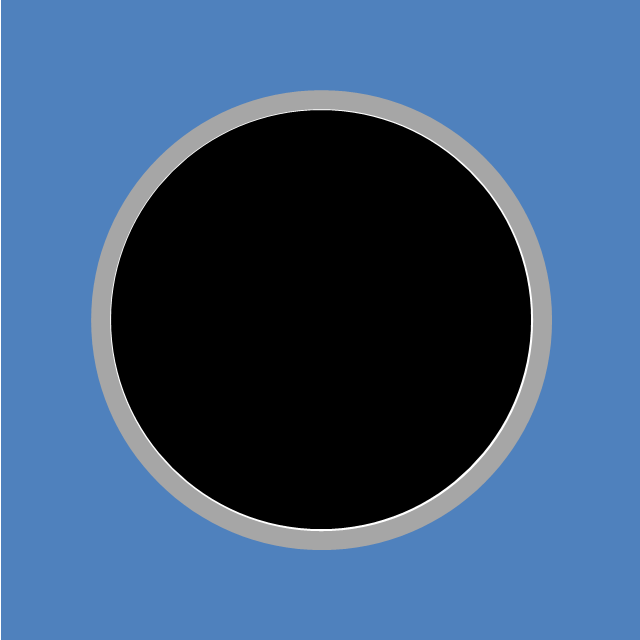
\includegraphics[width=\linewidth]{figures/pin_1.PNG}
		\caption{}
		\label{fig:pin-discretization-a}
	\end{subfigure}
	\begin{subfigure}{0.45\textwidth}
		\centering
		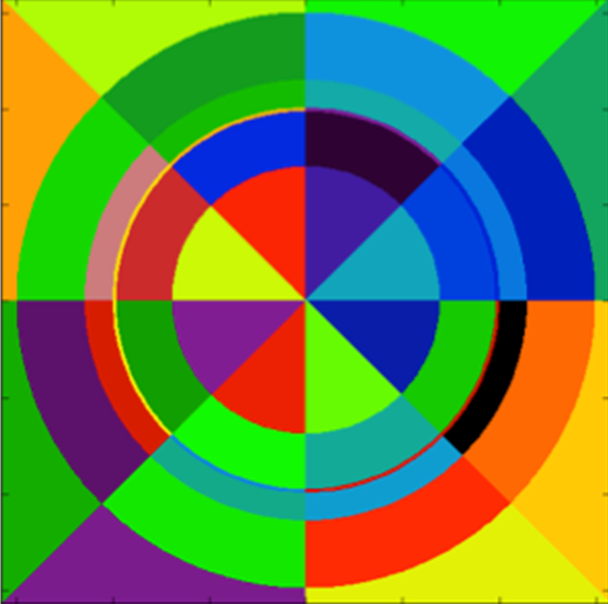
\includegraphics[width=\linewidth]{figures/pin_1_discretized.PNG}
		\caption{}
		\label{fig:pin-discretization-b}
	\end{subfigure}
	\caption[]{A description of source region discretization and mesh refinement. The geometry is shown (a) colored by material and (b) colored by source region.}
	\label{fig:pin-discretization}
\end{figure}

\section{Track Discretization of the MOC Equations}
\label{sec:track-disceretization}

\ac{MOC} discretizes the angular space by choosing a finite number of directions to lay down \textit{tracks} across the geometry. For each direction, tracks span the entire geometry between outer boundaries. A collection of tracks is termed the \textit{track laydown}. A radial view of a coarse track laydown for a simple pin-cell geometry is shown in Figure~\ref{fig:track-laydown}. The geometry is colored by material region; namely water, clad, gap, and fuel. Note that the final track laydown traverses tracks forward and backward, rather than generating tracks in each direction, for computational efficiency~\cite{kochunas2007twoway}.


\begin{figure}[h!]
	\centering
	\begin{subfigure}{0.3\textwidth}
		\centering
		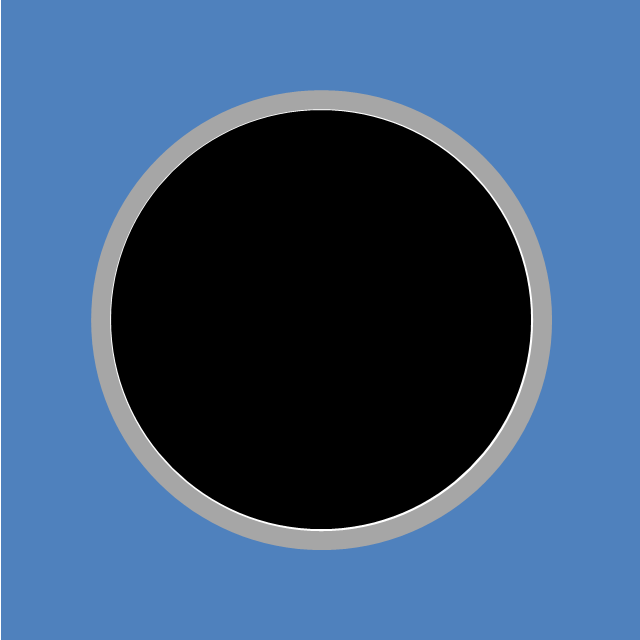
\includegraphics[width=\linewidth]{figures/pin_1.PNG}
		\caption{}
		\label{fig:track-laydown-a}
	\end{subfigure}
	\begin{subfigure}{0.3\textwidth}
		\centering
		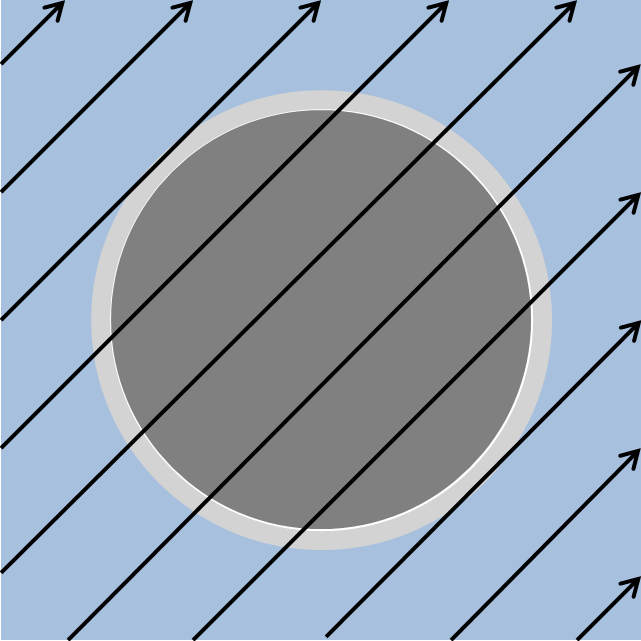
\includegraphics[width=\linewidth]{figures/pin_2.PNG}
		\caption{}
		\label{fig:track-laydown-b}
	\end{subfigure}
	\begin{subfigure}{0.3\textwidth}
		\centering
		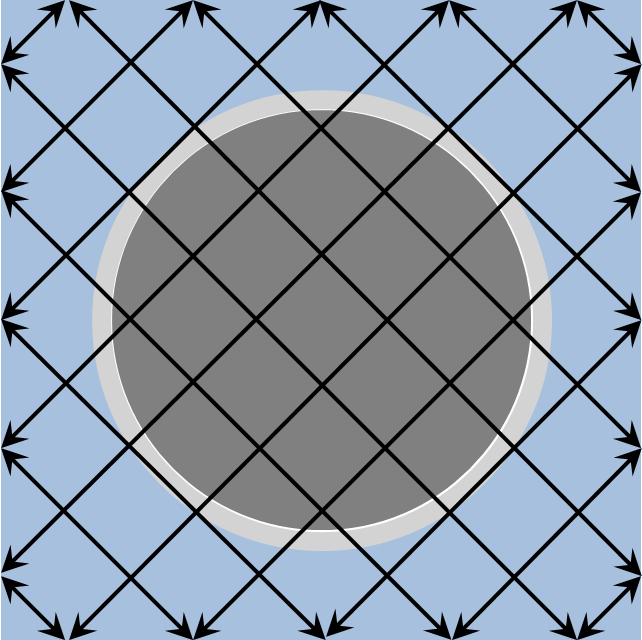
\includegraphics[width=\linewidth]{figures/pin_3.PNG}
		\caption{}
		\label{fig:track-laydown-c}
	\end{subfigure}
	\caption[]{A description of the track laydown process. The geometry (a) is shown followed by the track laydown (b) for one particular direction. Finally the entire track laydown for 4 azimuthal angles is shown (c) with arrows showing that each track is traversed both forward and backward. Note that the track laydowns shown here are significantly coarser than usual track laydowns for illustration purposes.}
	\label{fig:track-laydown}
\end{figure}

For each track crossing a given constant cross-section region, the variation of angular flux follows Eq.~\ref{eqn:moc-source-int}. Therefore, each track is discretized into \textit{segments}, in which each segment is the portion of the track that crosses a particular region. Across each segment, Eq.~\ref{eqn:moc-source-int} applies. An illustration of the segmentation process for the simple pin-cell geometry is shown in Figure~\ref{fig:segmentation}. The presented track, with the geometry drawn along its direction of travel is discretized into segments by material region. For simplicity, this illustration does not discretize the source regions further than material boundaries. A real segmentation process might discretize segments over the domain shown in Figure~\ref{fig:pin-discretization-b}. This process would treat all tracks shown in the track laydown (eg. Figure~\ref{fig:track-laydown}) in a similar manner. These images show track laydown and segmentation in just the radial plane, but the same methodology applies to three dimensional geometries.

\begin{figure}[h!]
	\centering
	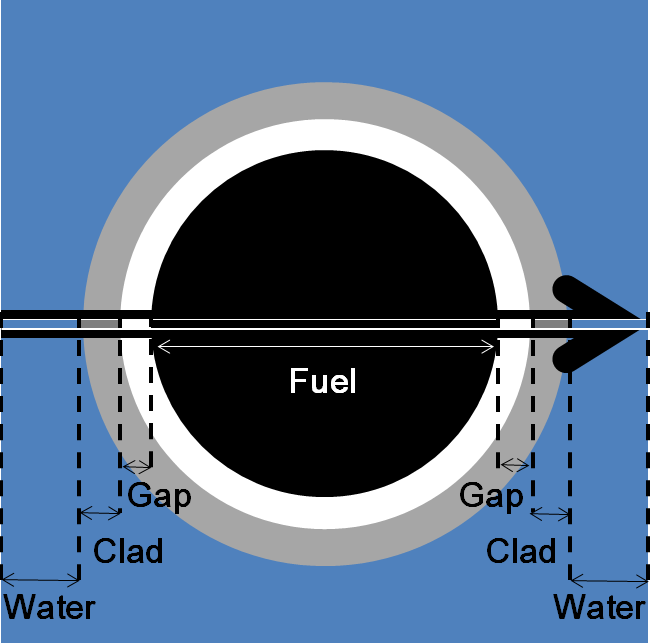
\includegraphics[width=0.6\linewidth]{figures/segmentation.PNG}
	\caption[]{The segmentation of a track horizontally traversing a pin-cell domain with coarse source discretization wherein the boundaries of source regions are no finer than their material region. The formed segments are colored by material region. For illustration purposes, the geometry is not shown to scale.}
	\label{fig:segmentation}
\end{figure}

Now that tracks have been segmented, a system of equations can be formed governing the variation of angular flux through each region as presented in Eq.~\ref{eqn:moc-source-int}. However, this expression has a dependence on the incoming angular flux. For segments originating in the bulk of the geometry, continuity of angular flux is naturally enforced. The outgoing flux of the preceding segment in the track provides the incoming flux of the segment. Specifically, the position-dependent angular flux $\psi_{p,g}^{t,\varsigma}(\mathbf{r})$ in group $g$ along track $t$ and segment $\varsigma$ can be expressed as the angular flux of the preceding segment $\varsigma-1$ at the interface point $\mathbf{r_{\textbf{int}}}$ where the segments meet as
\begin{dmath}
	\psi_{p,g}^{t,\varsigma}(\mathbf{r_{\textbf{int}}}) = \psi_{p,g}^{t,\varsigma-1}(\mathbf{r_{\textbf{int}}}).
\end{dmath}
Defining the angular flux along a segment in terms of distance traveled along the segment rather than position, this can equivalently be written as
\begin{dmath}
	\psi_g^{t,\varsigma}(0) = \psi_g^{t,\varsigma-1}(\ell_{t,\varsigma-1})
	\label{eqn:angular_flux_boundary}
\end{dmath}
where $\ell_{t,\varsigma}$ refers to the length of segment $\varsigma$ along track $t$. For angular fluxes originating at the geometry boundary, the boundary condition provides the relationship for the angular flux. 

%For vacuum boundary conditions, it is assumed that there is no impinging angular flux, so the incoming angular flux is simply taken to be zero at the boundary. 
For reflective boundary conditions, the incoming angular flux is equal to the outgoing angular flux of the reflected angle. This requires that a track be present with the correct reflecting angle, meeting at precisely the same point on the boundary. This is enforced during the track laydown, further discussed in Chapter~\ref{chap:track-laydown}.

%If only vacuum boundary conditions were present, this restriction on track laydown would not be necessary. Similar treatments are possible for periodic and rotational boundary conditions if enforced by the track laydown.  A more complete discussion of track laydown is given in Chapter~\ref{chap:track-laydown} and the conditions required to link tracks at geometric boundaries will be discussed at length.

%Precise definitions are needed in order to discuss the relation of these tracks to the \ac{MOC} equations. 

Tracks are defined to originate at one boundary and span the geometry until they terminate at another boundary. The segments of a track are ordered in the direction of the track so that only the first segment is affected by a boundary condition. Track $t$ is defined to have $S(t)$ segments. For vacuum boundaries,
\begin{dmath}
	\psi_g^{t,1}(0) = 0.
\end{dmath}
For boundary conditions (such as reflective, periodic, and rotational) that connect with another track, the function $C$ is defined which yields the linking track. For instance, the incoming angular flux of track $t$ would connect with the outgoing angular flux of track $C(t)$ as
\begin{dmath}
	\psi_g^{t,1}(0) = \psi_g^{C(t),S(C(t))}(\ell_{C(t),S(C(t))})
	\label{eqn:linking-bc}
\end{dmath}

With the angular and spatial discretization from the track laydown, the angular flux relationship along a characteristic path given in Eq.~\ref{eqn:moc-source-int} can be presented in terms of the discretized track segments in Eq.~\ref{eqn:gen-angular-flux-var-disc} where $i$ is the region traversed by track $t$ and segment $\varsigma$. 
\begin{dmath}
	\psi_g^{t,\varsigma}(s) = \psi^{t,\varsigma}_g(0) e^{-\Sigma_{t}^{i,g} s} + \int\displaylimits_{0}^{s} ds' \, e^{-\Sigma_{t}^{i,g} (s-s')}q_{t,\varsigma,g}(s)
	\label{eqn:gen-angular-flux-var-disc}
\end{dmath}
Note that when the transformation to distance $s$ is performed on the source, it also becomes dependent on the track segment even though the source is assumed to be isotropic. This is because the source can have a shape within the region and track segments traverse the region at different positions.

Still, these equations only determine the behavior of the neutron flux along a particular track. However, the region-averaged scalar flux is often desired. The average scalar flux $\overline{\phi_{i,g}}$ in a region $i$ for group $g$ can be computed by integrating over all directions as
\begin{dmath}
	\overline{\phi_{i,g}} = \frac{1}{V_i}\int_V dV \, \int_{4\pi} d\Omega \, \psi_g(\mathbf{r},\mathbf{\Omega}).
	\label{eqn:avg-flux-theory}
\end{dmath}
In order to numerically calculate the integral, each track represents a volume formed by the product of its length and both the radial and axial perpendicular distances to tracks of the same direction. Those perpendicular lengths form the track cross-sectional area as illustrated in Figure~\ref{fig:track-cross-section}. This illustration just shows the radial view of the tracks. However, in three dimensions, axial distances also exist between tracks, so the track cross-sectional area does indeed represent an area rather than a distance.
\begin{figure}[h!]
	\centering
	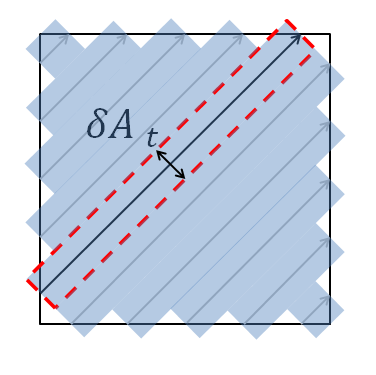
\includegraphics[width=0.6\linewidth]{figures/track-cross-sectional-area.PNG}
	\caption[]{An illustration of the spatial volume represented by each track as the product of track length and track cross-sectional area $\delta A_t$. The volume represented by each track is shaded in blue.}
	\label{fig:track-cross-section}
\end{figure}
With a fine track laydown, the discretization error becomes small. Similarly, each track $t$ has an angular weight $\alpha_t$ relating to the width of the angular space represented by the track. Therefore the overall weight of the track $w_t$ is calculated as the product of track cross-sectional area and angular weight as given in Eq.~\ref{eqn:weight-def}.
\begin{equation}
w_{t} = \delta A_{t} \alpha_t
\label{eqn:weight-def}
\end{equation}
With each track representing a discretized portion of the spatial and angular domain, Eq.~\ref{eqn:avg-flux-theory} can be transformed to reflect the track discretization in Eq.~\ref{eqn:average-flux-disc}, yielding a closed-form relationship to calculate the scalar flux.
\begin{dmath}
	\overline{\phi_{i,g}} = \frac{1}{V_i} \sum_{(t,\varsigma) \in V_i} w_{t} \int_{0}^{\ell_{t,\varsigma}} ds \, \psi^{t,\varsigma}_g(s)
	\label{eqn:average-flux-disc}
\end{dmath}

\section{Track Simplifications and Calculation of Volumes}
\label{sec:track-simplifications}

In the previous section, the track discretization of the \ac{MOC} equation was introduced. In the section, it was noted that tracks are used in both forward and backward directions. In the notation, a given track $t$ represents only a single direction. Due to the two directional tracks traversing the same line, simplifications can sometimes be made to the equations.

Consider the weighted summation of values $r_{t,\varsigma}$ which are potentially dependent on the traversed segment $\varsigma$ of track $t$. The summation can be cast as
\begin{equation}
	\sum_{(t,\varsigma) \in V_i} w_t r_{t,\varsigma} = \sum_{(t,\varsigma) \in V^F_i} w_t r_{t,\varsigma} + \sum_{(t,\varsigma) \in V^B_i} w_t r_{t,\varsigma}
\end{equation}
where $V^F_i$ refers to the volume tracked by forward traversed tracks and $V^B_i$ refers to the volume tracked by backward traversed tracks. Note that the corresponding forward/backward tracks have opposite directions. Therefore, if quantity $\tilde{r}_{t,\varsigma}$ does not depend on the direction $\mathbf{\Omega}$, then for any direction $v \in (x,y,z)$ and any \textit{odd} integer $d$,
\begin{equation}
\sum_{(t,\varsigma) \in V_i} w_t \left(\Omega_{v,t}\right)^d \tilde{r}_{t,\varsigma} = 0.
\end{equation}
Similarly, for any \textit{even} integer $d$,
\begin{equation}
\sum_{(t,\varsigma) \in V_i} w_t \left(\Omega_{v,t}\right)^d \tilde{r}_{t,\varsigma} = 2 \sum_{(t,\varsigma) \in V^F_i} \left(\Omega_{v,t}\right)^d w_t \tilde{r}_{t,\varsigma}.
\end{equation}
The calculation of region volumes is one example where this simplification can be used. In order for the \ac{MOC} equations to be accurate, the condition
\begin{dmath}
	\frac{1}{V_i} \sum_{(t,\varsigma) \in V_i} w_{t} \int_{0}^{\ell_{t,\varsigma}} ds \, 1 = 1
\end{dmath}
should apply. However, for a coarse track laydown the volume is not perfectly accurate, causing the condition not to be met. Therefore, volumes are calculated with the tracked lengths and weights as
\begin{dmath}
	V_i = \sum_{(t,\varsigma) \in V_i} w_{t} \ell_{t,\varsigma}
\end{dmath}
which forces the aforementioned condition to be met. This can be simplified by noting that $\ell_{t,\varsigma}$ is not dependent on direction, allowing the volume to be calculated only using forward-directed tracks as
\begin{equation}
V_i = 2 \sum_{(t,\varsigma) \in V^F_i} w_{t} \ell_{t,\varsigma}.
\end{equation}

\section{Flat Source Approximation}
\label{sec:flat-source}

One common low-order approximation for the neutron source is the flat source approximation. This approximation assumes the neutron source for a given energy group $q_g(\mathbf{r})$ is spatially constant over each source region. The flat source approximation is also the most frequently used approximation in standard \ac{MOC} solvers~\cite{dragon_3d_moc, kochunas, apollo3_vv, cactus_3d, liu_mrt, mockingbird, rhodes2006casmo}. For this approximation, the angular flux relationship given in Eq.~\ref{eqn:gen-angular-flux-var-disc} reduces to
\begin{dmath}
	\psi_g^{t,\varsigma}(s) = \psi^{t,\varsigma}_g(0) e^{-\Sigma_{t}^{i,g} s}  + \frac{q^0_{i,g}}{\Sigma_{t}^{i,g}} F_1 \left(\Sigma_{t}^{i,g}s\right)
	\label{eqn:angular-flux-var}
\end{dmath}
with region $i$ having constant neutron source $q^0_{i,g}$ where
\begin{equation}
F_1(\tau) = 1 - e^{-\tau}.
\label{eq:f1}
\end{equation}

This equation allows for the computation of all angular fluxes within a region of neutron source $q^0_{i,g}$. From the definition of the neutron source in Eq.~\ref{eqn:source}, the constant neutron source $q^0_{i,g}$ in the region $i$ can be computed as
\begin{equation}
q^0_{i,g} = \frac{1}{4 \pi} \left( \frac{\chi_{i,g}}{k} \sum_{g'=1}^{G} \nu_{i,g'} \Sigma_f^{i,g'} \overline{\phi_{i,g'}} + \, \sum_{g'=1}^G \,  \Sigma_{s}^{i,g' \rightarrow g} \overline{\phi_{i,g'}} \right)
\label{eqn:source-discr}
\end{equation}
where $\overline{\phi_{i,g}}$ is the average scalar flux in the region and the cross-sections have been taken to be constant over each region $i$. Combining Eq.~\ref{eqn:average-flux-disc} with Eq.~\ref{eqn:angular-flux-var}, the scalar flux can be calculated using the relationship in Eq.~\ref{eqn:average-flux}.
\begin{dmath}
	\overline{\phi_{i,g}} = \frac{q^0_{i,g}}{\Sigma_{t}^{i,g}} + \frac{1}{\Sigma_{t}^{i,g} V_i} \sum_{(t,\varsigma) \in V_i} w_{t} \left( \psi_g^{t,\varsigma}(0) - \psi_g^{t,\varsigma}(\ell_{t,\varsigma}) \right)
	\label{eqn:average-flux}
\end{dmath}
The calculated fluxes can then be used to construct the neutron sources $q^0_{i,g}$ for each region $i$ and each energy group $g$ with the relationship in Eq.~\ref{eqn:source-discr}. The solution of the \ac{MOC} system of equations is discussed in great detail in Appendix~\ref{app:matrix-moc}. It is important to note that the application of \ac{MOC} equations over all segments (Eq.~\ref{eqn:average-flux-disc} and Eq.~\ref{eqn:angular-flux-var}) for a given source distribution is termed a \textit{transport sweep}.


\section{Track-based Linear Source Approximation}
\label{sec:linear-source}

In the previous section, the MOC equations were derived using a flat source approximation. While this approximation is convenient and used by many, a linear approximation can potentially reduce the computational requirements of simulating a spatially converged reactor problem. While the linear source approximation increases the computational cost for a fixed discretization, the higher-order source can capture source gradients, allowing for a much coarser mesh discretization while maintaining solution accuracy~\cite{ferrer2012linear}. In this section, the track-based linear source approximation developed by Ferrer~\cite{ferrer2015linear} for 2D \ac{MOC} is extended to 3D \ac{MOC}. A discussion of the subtleties in the derivation and implementation is presented.


\subsection{Derivation of the Linear Source Approximation}

With a linear source approximation, the source is assumed to vary linearly over a given track $t$ on segment $\varsigma$ that traverses region $i$ as
\begin{equation}
q_{t,\varsigma,g}(s) = q^0_{t,\varsigma,g} + q^1_{t,\varsigma,g}(s-\ell_{t,\varsigma}/2)
\label{eq:track-ls}
\end{equation}
where $\ell_{t,\varsigma}$ is the length of the track $t$ over the region $i$ and the track-dependent coefficients are $q^0_{t,\varsigma,g}$ and $q^1_{t,\varsigma,g}$ . It is important to note that in this definition the source components are dependent on the track. Later, the track description of the source will be transformed into one dependent on only the source region, not on the track. For a linear source defined by the spatial region, the source for each track varies since tracks enter the source regions at different positions and different angles. This motivates track-dependent source components. 

By inserting the linear source definition into the balance equation, the angular flux follows the relationship
\begin{equation}
\psi_g^{t,\varsigma}(s) = \psi_g^{t,\varsigma}(0) e^{-\Sigma_{t}^{i,g} s} + \int\displaylimits_{0}^{s} ds' \, (q^0_{t,\varsigma,g} + q^1_{t,\varsigma,g}(s'-\ell_{t,\varsigma}/2)) e^{-\Sigma_{t}^{i,g} (s-s')}.
\label{eq:first-ls}
\end{equation}
In this form, it is possible to analytically calculate the angular flux variation along any track given the track-based linear source components. In the following subsections, the linear source equations will be derived starting from this equation and the definition of the linear source.

\subsubsection{Calculation of Average Scalar and Angular Fluxes}

The calculation of average scalar fluxes is often the goal of neutron transport simulations. Therefore, this derivation of the track-based linear source approximation starts with a discussion of their calculation given the linear source definition. The angular flux relationship previously presented in Eq.~\ref{eq:first-ls} can be simplified to
\begin{equation}
\psi_g^{t,\varsigma}(s) = \psi^{t,\varsigma}_g(0) + \left( \frac{q^0_{t,\varsigma,g}}{\Sigma_{t}^{i,g}} - \psi_g^{t,\varsigma}(0) \right) F_1\left(\Sigma_{t}^{i,g} s \right) + \left(\frac{q^1_{t,\varsigma,g}}{2\left(\Sigma_{t}^{i,g}\right)^2}\right) F_2\left(\Sigma_{t}^{i,g} s, \Sigma_{t}^{i,g} \ell_{t,\varsigma} \right)
\label{eq:ls-angular-flux}
\end{equation}
where the function $F_1$ follows the form given in Eq.~\ref{eq:f1} and $F_2$ is defined in terms of $F_1$ as
\begin{equation}
F_2(\tau_1, \tau_2) = 2 \left[\tau_1 - F_1(\tau_1)\right] - \tau_2 F_1(\tau_1)
\label{eq:f2}
\end{equation}
Recall that the average flux can be computed by integrating angular fluxes as presented in Eq.~\ref{eqn:average-flux-disc}. This can be re-written in terms of average angular fluxes as
\begin{equation}
\overline{\phi_{i,g}} = \frac{1}{V_i} \sum_{(t,\varsigma) \in V_i} w_t \overline{\psi}^{t,\varsigma}_g \ell_{t,\varsigma}
\label{eq:flat-scalar-flux}
\end{equation}
where the angular average angular flux $\overline{\psi}^{t,\varsigma}_g$ over a segment is defined by
\begin{equation}
\overline{\psi}^{t,\varsigma}_g = \frac{1}{\ell_{t,\varsigma}}\int_{0}^{\ell_{t,\varsigma}} ds \, \psi^{t,\varsigma}_g(s).
\end{equation}
After the MOC transform and with the linear source approximation, the neutron transport equation takes the form
\begin{equation}
\frac{d\psi_{i,g}(s)}{ds} \, + \, \Sigma_{t}^{i,g} \psi(s) = q^0_{t,\varsigma,g} + q^1_{t,\varsigma,g}(s-\ell_{t,\varsigma}/2)
\end{equation}
when the angular and spatial discretization is applied. This relationship can be rearranged to solve for the average angular flux $\overline{\psi}^{t,\varsigma}_g$ as
\begin{equation}
\overline{\psi}^{t,\varsigma}_g = \frac{q^0_{t,\varsigma,g}}{\Sigma_{t}^{i,g}} + \frac{\psi^{t,\varsigma}_g(0) - \psi^{t,\varsigma}_g(\ell_{t,\varsigma})}{\Sigma_{t}^{i,g} \ell_{t,\varsigma}}
\label{eq:ls-avg-angular-flux}
\end{equation}

From a neutron source definition presented in Eq.~\ref{eq:track-ls}, the angular fluxes and their segment averages can be calculated using Eq.~\ref{eq:ls-avg-angular-flux} with Eq.~\ref{eq:ls-angular-flux}, respectively. The scalar fluxes can also be computed by combining Eq.~\ref{eq:flat-scalar-flux} with Eq.~\ref{eq:ls-avg-angular-flux}, yielding
\begin{equation}
\overline{\phi_{i,g}} = \frac{1}{V_i} \sum_{(t,\varsigma) \in V_i} w_t \ell_{t,\varsigma} \left( \frac{q^0_{t,\varsigma,g}}{\Sigma_{t}^{i,g}} + \frac{\psi^{t,\varsigma}_g(0) - \psi^{t,\varsigma}_g(\ell_{t,\varsigma})}{\Sigma_{t}^{i,g} \ell_{t,\varsigma}} \right)
\end{equation}
which can be simplified as
\begin{equation}
\overline{\phi_{i,g}} = \frac{\overline{q}_{i,g}}{\Sigma_{t}^{i,g}} + \frac{1}{\Sigma_{t}^{i,g} V_i} \sum_{(t,\varsigma) \in V_i} w_t \left(\psi^{t,\varsigma}_g(0) - \psi^{t,\varsigma}_g(\ell_{t,\varsigma}) \right)
\label{eq:ls-avg-scalar-flux}
\end{equation}
which is the same analytic form as derived from the flat source approximation in Eq.~\ref{eqn:average-flux}.

%%%%%%%%%%%%%%%%%%%%%%%%%%%%%%%%%%%%%%%%%%%%%%%%%%%%%%%%%%%%%%%%%%%%%%%%%%%%%%%
\subsubsection{Linear Source Defined By Region}

Until now, the linear source approximation has been introduced in the perspective of each track. This is convenient for simplifying the MOC equations, but not convenient for computing region-dependent components. Therefore, a region-wise linear source $q_i^g$ for region $i$ and energy group $g$ is defined in terms of position $\mathbf{r}$ as
\begin{equation}
q_{i,g}(\mathbf{r}) = \overline{q}_{i,g} + \vec{q}_{i,g} \cdot \left( \mathbf{r} - \mathbf{r}^C_i \right)
\label{eq:ls-regional}
\end{equation}
where $\overline{q}_{i,g}$ is the flat source component, $\vec{q}_{i,g}$ is a vector representing the gradient of the source, and $\mathbf{r}^C_i$ is the centroid of the region $i$. The source gradient can be defined in terms of its components as $\vec{q}_{i,g} = \left[q_{x,i,g}, q_{y,i,g}, q_{z,i,g} \right]^T$ where $q_{x,i,g}$, $q_{y,i,g}$, and $q_{z,i,g}$ are the source gradients in the $x$, $y$, and $z$ directions, respectively. Here the vector notation $\vec{q}$ was chosen to avoid confusion with $\mathbf{q}$, the vector of all sources across all regions and energy groups. With this formalism, the track-based linear source components defined in Eq.~\ref{eq:track-ls} can be computed as:
\begin{equation}
q^0_{t,\varsigma,g} = q_{i,g}(\mathbf{r}^m_{t,\varsigma}) = \overline{q}_{i,g} + \vec{q}_{i,g} \cdot \left( \mathbf{r}^m_{t,\varsigma} - \mathbf{r}^C_i \right)
\end{equation}
\begin{equation}
q^1_{t,\varsigma,g} = \vec{q}_{i,g} \cdot \mathbf{\Omega}_t
\end{equation}
where $\mathbf{r}^m_{t,\varsigma}$ is the midpoint of segment $\varsigma$ along track $t$ and $\mathbf{\Omega}_t$ is its unit vector direction. In Cartesian coordinates, the source defined in Eq.~\ref{eq:ls-regional} can be defined as
\begin{equation}
q_{i,g}(x, y, z) = \overline{q}_{i,g} + q_{x,i,g} \left( x - x^C_i \right) + q_{y,i,g} \left( y - y^C_i \right) + q_{z,i,g} \left( z - z^C_i \right)
\end{equation}
where $x^C_i$, $y^C_i$, and $z^C_i$ represent the $x$, $y$, and $z$ coordinates of the region $i$ centroid, respectively. The centroid represents the midpoint of the cell, as observed by traversing segments. The source can be written more compactly as
\begin{equation}
q_{i,g}(x, y, z) = \overline{q}_{i,g} + \sum_{v \in (x,y,z)} q_{v,i,g} \left( v - v^C_i \right)
\end{equation}
where $v$ represents the spatial variables $x$, $y$, and $z$. Using this notation, the track-based source components can be expressed as:
\begin{equation}
q^0_{t,\varsigma,g} = \overline{q}_{i,g} + \sum_{v \in (x,y,z)} q_{v,i,g} \left( v^m_{t,\varsigma} - v^C_i \right)
\label{eq:q0-def}
\end{equation}
\begin{equation}
q^1_{t,\varsigma,g} = \sum_{v \in (x,y,z)} \Omega_{v,t} q_{v,i,g}
\label{eq:q1-def}
\end{equation}
where $\Omega_{v,t}$ refers to the $v\in(x,y,z)$ component of the unit vector direction $\mathbf{\Omega}_t$ for track $t$ and $v^m_{t,\varsigma}$ refers to the $v$ coordinate of the midpoint of segment $\varsigma$ along track $t$. The $v$ coordinate of the centroid, $v^C_i$, can be computed as
\begin{equation}
v^C_i = \sum_{(t,\varsigma) \in V_i} w_t \int_{0}^{\ell_{t,\varsigma}} ds \, v \qquad \forall v \in (x,y,z).
\label{eq:gen-centroid-int}
\end{equation}
The variables $x$, $y$, and $z$ corresponding to $v$ can be cast in terms of the distance $s$ along a segment as
\begin{equation}
v = v^m_{t,\varsigma} + \Omega_{v,t} \left(s - \frac{\ell_{t,\varsigma}}{2} \right) \qquad \forall v \in (x,y,z)
\label{eq:v-to-s}
\end{equation}
which can be inserted in Eq.~\ref{eq:gen-centroid-int} to yield the simplified form as
\begin{equation}
v^C_i = \sum_{(t,\varsigma) \in V_i} w_t \ell_{t,\varsigma} v^m_{t,\varsigma} \qquad \forall v \in (x,y,z).
\label{eq:gen-centroid-sum}
\end{equation}
The flat source component $\overline{q}_{i,g}$ can be computed using the scalar fluxes in the same way as the flat source approximation,
\begin{equation}
\overline{q}_{i,g} = \frac{1}{4 \pi} \left( \frac{\chi_{i,g}}{k} \sum_{g'=1}^{G} \nu_{i,g'} \Sigma_f^{i,g'} \overline{\phi_{i,g'}} + \, \sum_{g'=1}^G \,  \Sigma_{s}^{i,g' \rightarrow g} \overline{\phi_{i,g'}} \right).
\label{eq:ls-flat-source}
\end{equation}

\subsubsection{Relating Linear Source Components To Moments}
\label{sec:ls-components}

With the neutron source defined in terms of spatial variables rather than track-based variables, it is possible to relate the linear source components to source moments. The moment $Q_{v,i,g}$ of the source in the $v\in(x,y,z)$ direction can be calculated as
\begin{equation}
Q_{v,i,g} = \int_{V_i} d\mathbf{r} \, \left(v - v^C_i\right) q(\mathbf{r}) \qquad \forall v \in (x,y,z)
\end{equation}
where $V_i$ is the volume of region $i$. With the track discretization, the integral can be calculated as
\begin{equation}
Q_{v,i,g}  = \sum_{(t,\varsigma) \in V_i} w_t \int_{0}^{\ell_{t,\varsigma}} ds \, \left(v - v^C_i\right) \left(\overline{q}_{i,g} + \sum_{v' \in (x,y,z)} q_{v',i,g} \left( v' - {v'}^C_i \right)\right) \qquad \forall v \in (x,y,z).
\end{equation}
This can be separated as
\begin{dmath}
	Q_{v,i,g} = \sum_{(t,\varsigma) \in V_i} w_t \int_{0}^{\ell_{t,\varsigma}} ds \, \left(v - v^C_i\right) \overline{q}_{i,g} + \\ {\sum_{(t,\varsigma) \in V_i} w_t \int_{0}^{\ell_{t,\varsigma}} ds \, \left(v - v^C_i\right) \left(\sum_{v' \in (x,y,z)} q_{v',i,g} \left( v' - {v'}^C_i \right)\right) \quad \forall v \in (x,y,z)}
\end{dmath}
and simplified to
\begin{equation}
Q_{v,i,g}  = \sum_{(t,\varsigma) \in V_i} w_t \int_{0}^{\ell_{t,\varsigma}} ds \, \left(v - v^C_i\right) \left(\sum_{v' \in (x,y,z)} q_{v',i,g} \left( v' - {v'}^C_i \right)\right) \qquad \forall v \in (x,y,z)
\label{eq:ls-source-moments}
\end{equation}
due to the definition of the region centroid in Eq.~\ref{eq:gen-centroid-int}. Defining moment coefficients $M_{v,v'}$ such that
\begin{equation}
M_{i,v,v'} = \sum_{(t,\varsigma) \in V_i} w_t  \int_{0}^{\ell_{t,\varsigma}} ds \, \left(v - v^C_i\right) \left( v' - {v'}^C_i \right) \qquad \forall (v,v') \in (x,y,z) \times (x,y,z),
\label{eq:moment-matrix-comp}
\end{equation}
it becomes clear that this can be cast as a linear problem such that
\begin{equation}
M_i \vec{q}_{i,g} = \vec{Q}_{i,g}
\label{eq:lin-moment-system}
\end{equation}
where $\vec{Q}_{i,g} = \left[Q_{x,i,g}, Q_{y,i,g}, Q_{z,i,g}\right]^T$ and the matrix $M_i$ is defined by Eq.~\ref{eq:moment-matrix-comp} where
\begin{equation}
M_i = 
\begin{bmatrix}
M_{i,xx} & M_{i,xy}  & M_{i,xz} \\
M_{i,xy} & M_{i,yy}  & M_{i,yz} \\
M_{i,xz} & M_{i,yz}  & M_{i,zz}
\end{bmatrix}.
\label{eq:linear-moment-matrix}
\end{equation}
Altogether, the linear system is defined by
\begin{equation}
\begin{bmatrix}
M_{i,xx} & M_{i,xy}  & M_{i,xz} \\
M_{i,xy} & M_{i,yy}  & M_{i,yz} \\
M_{i,xz} & M_{i,yz}  & M_{i,zz}
\end{bmatrix}
\begin{bmatrix}
q_{x,i,g} \\
q_{y,i,g} \\
q_{z,i,g}
\end{bmatrix}
=
\begin{bmatrix}
Q_{x,i,g} \\
Q_{y,i,g} \\
Q_{z,i,g}
\end{bmatrix}
.
\label{eq:moments-linear-sys}
\end{equation}
The source moments can then be calculated similarly to the flat source components, using the relationship
\begin{equation}
Q_{v,i,g} = \frac{1}{4 \pi} \left( \frac{\chi_{i,g}}{k} \sum_{g'=1}^{G} \nu_{i,g'} \Sigma_f^{i,g'} \hat{\phi}_{v,i,g'} + \, \sum_{g'=1}^G \,  \Sigma_{s}^{i,g' \rightarrow g} \hat{\phi}_{v,i,g'} \right) \qquad \forall v \in (x,y,z)
\end{equation}
where $\hat{\phi}_{v,i,g}$ is the moment of the scalar flux in the $v$ direction. These scalar fluxes can be computed in parallel over all regions based on scalar flux moments.


\subsubsection{Calculation of Scalar Flux Moments}
\label{sec:ls-moments}
The previous section allowed for the calculation of linear source moments given scalar flux moments. These scalar flux moments can be calculated by
\begin{equation}
\hat{\phi}_{v,i,g} = \sum_{(t,\varsigma) \in V_i} w_t \int_{0}^{\ell_{t,\varsigma}} ds \, \left(v - v^C_i\right) \psi^{t,\varsigma}_g(s) \qquad \forall v \in (x,y,z).
\end{equation}
Converting the variable $v$ into the tracked distance $s$ using Eq.~\ref{eq:v-to-s}, this can be recast as
\begin{equation}
\hat{\phi}_{v,i,g} = \sum_{(t,\varsigma) \in V_i} w_t \int_{0}^{\ell_{t,\varsigma}} ds \, \left[v^m_{t,\varsigma} + \Omega_{v,t} \left(s - \frac{\ell_{t,\varsigma}}{2} \right) - v^C_i \right] \psi^{t,\varsigma}_g(s) \qquad \forall v \in (x,y,z)
\end{equation}
and simplified to
\begin{equation}
\hat{\phi}_{v,i,g} = \sum_{(t,\varsigma) \in V_i} w_t \ell_{t,\varsigma} \left[\Omega_{v,t} \hat{\psi}^{t,\varsigma}_g +  \left( v^m_{t,\varsigma}- v^C_i - \frac{\Omega_{v,t} \ell_{t,\varsigma}}{2} \right) \overline{\psi}^{t,\varsigma}_g \right] \qquad \forall v \in (x,y,z)
\label{eq:flux-moments-1}
\end{equation}
where $\overline{\psi}^{t,\varsigma}_g$ is the average angular flux which can be calculated using Eq.~\ref{eq:ls-avg-angular-flux} and $ \hat{\psi}^{t,\varsigma}_g$ is the angular flux moment defined by
\begin{equation}
\hat{\psi}^{t,\varsigma}_g = \int_{0}^{\ell_{t,\varsigma}} ds \, s \psi^{t,\varsigma}_g(s).
\end{equation}
To solve for the angular flux moment, the definition for angular flux in Eq.~\ref{eq:ls-angular-flux} is inserted, yielding
\begin{equation}
\hat{\psi}^{t,\varsigma}_g = \int_{0}^{\ell_{t,\varsigma}} ds \, s \left(\psi^{t,\varsigma}_g(0) + \left( \frac{q^0_{t,\varsigma,g}}{\Sigma_{t}^{i,g}} - \psi_g^{t,\varsigma}(0) \right) F_1\left(\Sigma_{t}^{i,g} s \right) + \left(\frac{q^1_{t,\varsigma,g}}{2\left(\Sigma_{t}^{i,g}\right)^2}\right) F_2\left(\Sigma_{t}^{i,g} s, \Sigma_{t}^{i,g} \ell_{t,\varsigma} \right)\right)
\end{equation}
which can be simplified to
\begin{equation}
\hat{\psi}^{t,\varsigma}_g = \frac{\psi^{t,\varsigma}_g(0) \ell_{t,\varsigma}}{2} + \left(\frac{q^0_{t,\varsigma,g}}{\Sigma_{t}^{i,g}} - \psi^{t,\varsigma}_g(0) \right) \frac{G_1(\Sigma_{t}^{i,g} \ell_{t,\varsigma})}{\Sigma_{t}^{i,g}} + \frac{\ell_{t,\varsigma} q^1_{t,\varsigma,g} G_2(\Sigma_{t}^{i,g} \ell_{t,\varsigma})}{2\left(\Sigma_{t}^{i,g}\right)^2}
\label{eq:angular-flux-moment}
\end{equation}
where the functions $G_1(\tau)$ and $G_2(\tau)$ are mathematically defined as
\begin{equation}
G_1(\tau) = 1 + \frac{\tau}{2} - \left(1 + \frac{1}{\tau}\right) F_1(\tau)
\end{equation}
and
\begin{equation}
G_2(\tau) = \frac{2}{3} \tau - \left(1 + \frac{2}{\tau}\right) G_1(\tau).
\end{equation}
With these definitions, the scalar flux moments can be calculated by inserting the definitions of average angular flux $\overline{\psi}^{t,\varsigma}_g$ (Eq.~\ref{eq:ls-avg-angular-flux}) and angular flux moments $\hat{\psi}^{t,\varsigma}_g$ (Eq.~\ref{eq:angular-flux-moment})  into the definition of the scalar flux moments in Eq.~\ref{eq:flux-moments-1}. This results in a long expression which, for simplicity, can be decomposed into four terms as
\begin{equation}
\hat{\phi}_{v,i,g} = K_1 + K_2 + K_3 + K_4
\end{equation}
where the terms are defined by:
\begin{align}
K_1 = & \frac{1}{\Sigma_{t}^{i,g}} \sum_{(t,\varsigma) \in V_i} w_t \ell_{t,\varsigma} q^0_{t,\varsigma,g} \left(\frac{\Omega_{v,t} G_1(\Sigma_{t}^{i,g} \ell_{t,\varsigma})}{\Sigma_{t}^{i,g}} +  v^m_{t,\varsigma} - v^C_i - \frac{\Omega_{v,t} \ell_{t,\varsigma}}{2} \right) \\
K_2 = & \frac{1}{\Sigma_{t}^{i,g}} \sum_{(t,\varsigma) \in V_i} w_t \Omega_{v,t} \ell_{t,\varsigma} \psi^{t,\varsigma}_g(0) \left(\frac{\Sigma_{t}^{i,g} \ell_{t,\varsigma}}{2} - G_1(\Sigma_{t}^{i,g} \ell_{t,\varsigma}) \right) \\
K_3 = & \frac{1}{2\left(\Sigma_{t}^{i,g}\right)^2} \sum_{(t,\varsigma) \in V_i} w_t q^1_{t,\varsigma,g} \Omega_{v,t} \ell_{t,\varsigma}^2 G_2(\Sigma_{t}^{i,g} \ell_{t,\varsigma}) \\
K_4 = & \frac{1}{\Sigma_{t}^{i,g}} \sum_{(t,\varsigma) \in V_i} w_t \left( v^m_{t,\varsigma} - v^C_i- \frac{\Omega_{v,t} \ell_{t,\varsigma}}{2} \right) \left(\psi^{t,\varsigma}_g(0) - \psi^{t,\varsigma}_g(\ell_{t,\varsigma}) \right)
\end{align}
Each of the terms can be simplified. First, $K_1$ can be simplified by inserting the definition of $q^0_{t,\varsigma,g}$ from Eq.~\ref{eq:q0-def}. After expanding terms, $K_1$ can be cast as
\begin{equation}
\begin{split}
K_1 = &\frac{\overline{q}_{i,g}}{\Sigma_{t}^{i,g}} \sum_{(t,\varsigma) \in V_i} w_t \ell_{t,\varsigma} \left(v^m_{t,\varsigma} - v^C_i \right) + 
\frac{\overline{q}_{i,g}}{\Sigma_{t}^{i,g}} \sum_{(t,\varsigma) \in V_i} w_t \Omega_{v,t} \ell_{t,\varsigma} \left[\frac{G_1(\Sigma_{t}^{i,g} \ell_{t,\varsigma})}{\Sigma_{t}^{i,g}} - \frac{\ell_{t,\varsigma}}{2}\right] + \\
& \frac{1}{\Sigma_{t}^{i,g}} \sum_{p \in (x,y,z)} q_{p,i,g} \sum_{(t,\varsigma) \in V_i} w_t \ell_{t,\varsigma} \left( p^m_{t,\varsigma} - p^C_i \right) \left[\frac{\Omega_{v,t} G_1(\Sigma_{t}^{i,g} \ell_{t,\varsigma})}{\Sigma_{t}^{i,g}} +  v^m_{t,\varsigma} - v^C_i - \frac{\Omega_{v,t} \ell_{t,\varsigma}}{2} \right]
\end{split}
\end{equation}
Note that the first term of $K_1$ is zero due to the definition of the centroid in Eq.~\ref{eq:gen-centroid-sum}. The second term also becomes zero by noting that all tracks are traversed forwards and backwards, utilizing the simplification discussed in Section~\ref{sec:track-simplifications}. Therefore, after further expanding terms, $K_1$ is simplified to 
\begin{equation}
\begin{split}
K_1 = & \frac{1}{\Sigma_{t}^{i,g}} \sum_{p \in (x,y,z)} q_{p,i,g} \sum_{(t,\varsigma) \in V_i} w_t \ell_{t,\varsigma} \left( p^m_{t,\varsigma} - p^C_i \right) \left(v^m_{t,\varsigma} - v^C_i\right) + \\
& \frac{1}{\Sigma_{t}^{i,g}} \sum_{p \in (x,y,z)} q_{p,i,g} \sum_{(t,\varsigma) \in V_i} w_t \Omega_{v,t} \ell_{t,\varsigma} \left( p^m_{t,\varsigma} - p^C_i \right) \left[\frac{G_1(\Sigma_{t}^{i,g} \ell_{t,\varsigma})}{\Sigma_{t}^{i,g}} - \frac{\ell_{t,\varsigma}}{2} \right]. \\
\end{split}
\end{equation}
Notice that the bracketed quantity in the second term is not dependent on direction. Therefore, by again utilizing the forward and backward tracking relationships discussed in Section~\ref{sec:track-simplifications}, the first term can be simplified and the second term can be eliminated, resulting in
\begin{equation}
K_1 = \frac{2}{\Sigma_{t}^{i,g}} \sum_{p \in (x,y,z)} q_{p,i,g} \sum_{(t,\varsigma) \in V^F_i} w_t \ell_{t,\varsigma} \left( p^m_{t,\varsigma} - p^C_i \right) \left(v^m_{t,\varsigma} - v^C_i\right)
\end{equation}
where $V^F_i$ represents the forward tracked volume of $V_i$, therefore using only half of the directional tracks. Next, $K_2$ can be simplified to
\begin{equation}
K_2 = \frac{1}{\Sigma_{t}^{i,g}} \sum_{(t,\varsigma) \in V_i} w_t \Omega_{v,t} \ell_{t,\varsigma} \psi^{t,\varsigma}_g(0) H(\Sigma_{t}^{i,g} \ell_{t,\varsigma})
\end{equation}
by defining the function $H$ as
\begin{equation}
H(\tau) = \frac{\tau}{2} - G_1(\tau).
\label{eq:h}
\end{equation}
The $K_3$ term can be simplified by inserting the definition of $q^1_{t,\varsigma,g}$ in Eq.~\ref{eq:q1-def} and again using the forward and backward tracking relationships discussed in Section~\ref{sec:track-simplifications} as
\begin{equation}
K_3 = \frac{1}{\left(\Sigma_{t}^{i,g}\right)^2} \sum_{p \in (x,y,z)} q_{p,i,g} \sum_{(t,\varsigma) \in V^F_i} w_t \Omega_{v,t} \Omega_{p,t} \ell_{t,\varsigma}^2 G_2(\Sigma_{t}^{i,g} \ell_{t,\varsigma}).
\end{equation}
The fourth and final term $K_4$ can be simplified as
\begin{equation}
K_4 = \frac{1}{\Sigma_{t}^{i,g}} \sum_{(t,\varsigma) \in V_i} w_t v^{\textbf{in}}_{t,\varsigma} \left(\psi^{t,\varsigma}_g(0) - \psi^{t,\varsigma}_g(\ell_{t,\varsigma}) \right)
\end{equation}
by defining the entering coordinate $v^{\textbf{in}}_{t,\varsigma}$ of the segment on the source region relative to the centroid as
\begin{equation}
v^{\textbf{in}}_{t,\varsigma} = v^m_{t,\varsigma} - v^C_i - \frac{\Omega_{v,t} \ell_{t,\varsigma}}{2}.
\end{equation}
Altogether, these equations can be combined and written compactly as
\begin{equation}
\begin{split}
\hat{\phi}_{v,i,g} = \frac{1}{\Sigma_{t}^{i,g}} \Bigg( q_{x,i,g} C_{v,x}^{i,g} + & q_{y,i,g} C_{v,y}^{i,g} + q_{z,i,g} C_{v,z}^{i,g} \Bigg)+  \\
\frac{1}{\Sigma_{t}^{i,g}} \sum_{(t,\varsigma) \in V_i} w_t & \left[\Omega_{v,t} \ell_{t,\varsigma} \psi^{t,\varsigma}_g(0) H(\Sigma_{t}^{i,g} \ell_{t,\varsigma}) + v^{\textbf{in}}_{t,\varsigma} \left(\psi^{t,\varsigma}_g(0) - \psi^{t,\varsigma}_g(\ell_{t,\varsigma}) \right)\right]
\end{split}
\label{eq:final-scalar-flux-moments}
\end{equation}
where for $v, p \in (x,y,z) \times (x,y,z)$
\begin{equation}
C_{v,p}^{i,g} =  2 \sum_{(t,\varsigma) \in V^F_i} w_t \ell_{t,\varsigma}^2 \Omega_{v,t} \Omega_{p,t} G_2(\Sigma_{t}^{i,g} \ell_{t,\varsigma}) + \frac{1}{\Sigma_{t}^{i,g}} \sum_{(t,\varsigma) \in V^F_i} w_t \ell_{t,\varsigma} \left( p^m_{t,\varsigma} - p^C_i \right) \left(v^m_{t,\varsigma} - v^C_i\right).
\label{eq:ls-C}
\end{equation}
The equations derived in this section form the basis of the linear source \ac{MOC} algorithm.

\section{MOC Algorithm with Linear Sources}
\label{sec:ls-algorithm}

The linear source equations are much more complex and greater in number than the flat source equivalent, so this section will highlight the important equations and discuss how to implement an algorithm.

\subsection{Identifying Invariant Constants}

Before starting transport sweeps, it is important to identify constants which are not dependent on iterative estimates of scalar and angular fluxes. These constants can be computed and re-used at each iteration. These constants must not consume too much memory or else their storage may have significant computational drawbacks. In the context of \ac{MOC}, since the number of segments is often significantly larger than the number of regions, explicit storage should be implemented for region-dependent constants and not for segment-dependent constants.

One example of region dependent constants that should be stored are the $C_{v,p}^{i,g}$ terms defined in Eq.~\ref{eq:ls-C}. Note these constants are solely dependent on the geometry and track laydown which are invariant over the iterative process. These constants are therefore computed and stored for every region $i$.

In addition, the computation of linear source components involves solving the system described in Eq.~\ref{eq:lin-moment-system},
\begin{equation*}
M_i \vec{q}_{i,g} = \vec{Q}_{i,g}
\end{equation*}
for every region $i$ and energy group $g$ where $\vec{q}_{i,g} = \left[q_{x,i,g}, q_{y,i,g}, q_{z,i,g} \right]^T$ and $\vec{Q}_{i,g} = \left[Q_{x,i,g}, Q_{y,i,g}, Q_{z,i,g}\right]^T$. The matrix $M_i$ which is a $3 \times 3$ matrix for every region $i$ represented in Eq.~\ref{eq:linear-moment-matrix} by
\begin{equation*}
M_i = 
\begin{bmatrix}
M_{i,xx} & M_{i,xy}  & M_{i,xz} \\
M_{i,xy} & M_{i,yy}  & M_{i,yz} \\
M_{i,xz} & M_{i,yz}  & M_{i,zz}
\end{bmatrix}
\end{equation*}
and the matrix components are computed with Eq.~\ref{eq:moment-matrix-comp} as:
\begin{equation*}
M_{i,v,v'} = \sum_{(t,\varsigma) \in V_i} w_t  \int_{0}^{\ell_{t,\varsigma}} ds \, \left(v - v^C_i\right) \left( v' - {v'}^C_i \right) \qquad \forall (v,v') \in (x,y,z) \times (x,y,z)
\end{equation*}
Note that these terms, and therefore also $M_i^{-1}$, are invariant and the explicit computation and storage of $M_i^{-1}$ is performed for every region.

The computation of $M_i^{-1}$ should be handled with great care. For regions that are thin in a particular Cartesian direction (for instance the $x$ direction), the associated moments in that direction can also become very small. For instance, a region thin in the $x$ direction can have extremely small $M_{i,xx}$. This can cause the matrix to be poorly conditioned. In OpenMOC, this is handled by treating thin regions in which the single direction moments (such as $M_{i,xx}$) are small ($ < 10^{-4} \textit{cm}^2$) as having spatially constant source in the thin direction. In the case of a thin $x$ direction, instead of handling the full $3 \times 3$ matrix, the system is simplified to a $2 \times 2$ matrix as
\begin{equation*}
M_i^{-1} = 
\begin{bmatrix}
\begin{matrix}
0  
\end{matrix}
& \begin{matrix} 
0\phantom{M_{i,yy}}  & 0\phantom{M_{i,yz}}
\end{matrix} \\
\begin{matrix} 
0 \\ 0 
\end{matrix}
& \begin{bmatrix}
M_{i,yy}  & M_{i,yz} \\
M_{i,yz}  & M_{i,zz}
\end{bmatrix}^{-1}
\end{bmatrix}
\end{equation*}
which is solved to determine the $y$ and $z$ linear source components and the $x$ component of the linear source is assumed to be zero. Similar simplifications are handled for thin $y$ and thin $z$ directions with the elimination of rows and columns involving the variable. If two directions are thin, then the source in both directions is treated as flat, with a simple $1\times1$ system evaluated to determine the source in the third direction. For example, for a region thin in both $x$ and $y$, the system reduces to
\begin{equation*}
M_i^{-1} = 
\begin{bmatrix}
0 & 0  & 0 \\
0 & 0  & 0 \\
0 & 0  & 1 / M_{i,zz}
\end{bmatrix}
\end{equation*}
which is used to form the source in the $z$ direction. For a region thin in all Cartesian directions, it is treated as having a flat source. In the linear source framework this means setting all elements of $M_i^{-1}$ to zero.

In addition to region-dependent terms, the functions $F_1$, $F_2$, and $H$ often arise in the \ac{MOC} equations. These terms are dependent on optical path length and therefore are segment and group-dependent. Therefore, they are not explicitly stored since the storage requirements would be computationally infeasible. Instead, they are computed on-the-fly, often through interpolation. This will be further discussed in Chapter~\ref{chap:software-design}.

\subsection{Transport Sweeps}

Before each transport sweep, the source moments $Q_{v,i,g}$ can be computed from scalar flux moments using Eq.~\ref{eq:ls-source-moments} as:
\begin{equation*}
Q_{v,i,g} = \frac{1}{4 \pi} \left( \frac{\chi_{i,g}}{k} \sum_{g'=1}^{G} \nu_{i,g'} \Sigma_f^{i,g'} \hat{\phi}_{v,i,g'} + \, \sum_{g'=1}^G \,  \Sigma_{s}^{i,g' \rightarrow g} \hat{\phi}_{v,i,g'} \right) \qquad \forall v \in (x,y,z)
\end{equation*}
These moments are then used with Eq.~\ref{eq:lin-moment-system} as
\begin{equation*}
\vec{q}_{i,g} = M_i^{-1} \vec{Q}_{i,g}
\end{equation*}
Recall that the $M_i^{-1}$ matrices are explicitly computed and stored before iterations. Therefore, the matrix values are simply loaded and only a matrix-vector multiplication is necessary during the computation of source components. The flat source components can then be computed in the same way as flat source \ac{MOC} using Eq.~\ref{eq:ls-flat-source} as
\begin{equation*}
\overline{q}_{i,g} = \frac{1}{4 \pi} \left( \frac{\chi_{i,g}}{k} \sum_{g'=1}^{G} \nu_{i,g'} \Sigma_f^{i,g'} \overline{\phi_{i,g'}} + \, \sum_{g'=1}^G \,  \Sigma_{s}^{i,g' \rightarrow g} \overline{\phi_{i,g'}} \right).
\end{equation*}
The angular fluxes $\psi_g^{t,\varsigma}$ can be computed using Eq.~\ref{eq:ls-angular-flux} as
\begin{equation*}
	\psi_g^{t,\varsigma}(s) = \psi_g^{t,\varsigma}(0) + \left( \frac{q^0_{t,\varsigma,g}}{\Sigma_{t}^{i,g}} - \psi_g^{t,\varsigma}(0) \right) F_1\left(\Sigma_{t}^{i,g} s \right) + \left(\frac{q^1_{t,\varsigma,g}}{2\left(\Sigma_{t}^{i,g}\right)^2}\right) F_2\left(\Sigma_{t}^{i,g} s, \Sigma_{t}^{i,g} \ell_{t,\varsigma} \right)
\end{equation*}
where the track-based flat source $q^0_{t,\varsigma,g}$ and the track-based linear source $q^1_{t,\varsigma,g}$ are evaluated using Eq.~\ref{eq:q0-def} and Eq.~\ref{eq:q1-def}:
\begin{equation}
	\nonumber
	q^0_{t,\varsigma,g} = \overline{q}_{i,g} + \sum_{v \in (x,y,z)} q_{v,i,g} \left( v^m_{t,\varsigma} - v^C_i \right)
\end{equation}

\begin{equation}
	\nonumber
	q^1_{t,\varsigma,g} = \sum_{v \in (x,y,z)} \Omega_{v,t} q_{v,i,g}
\end{equation}
The scalar fluxes $\overline{\phi_{i,g}}$ and flux moments $\hat{\phi}_{v,i,g}$ can therefore be calculated with Eq.~\ref{eq:ls-avg-scalar-flux} and Eq.~\ref{eq:final-scalar-flux-moments}:
\begin{equation}
\nonumber
\overline{\phi_{i,g}} = \frac{\overline{q}_{i,g}}{\Sigma_{t}^{i,g}} + \frac{1}{\Sigma_{t}^{i,g} V_i} \sum_{(t,\varsigma) \in V_i} w_t \left(\psi^{t,\varsigma}_g(0) - \psi^{t,\varsigma}_g(\ell_{t,\varsigma}) \right)
\label{eq:ls-avg-scalar-flux-iter}
\end{equation}
\begin{equation}
\nonumber
\begin{split}
\hat{\phi}_{v,i,g} = \frac{1}{\Sigma_{t}^{i,g}} \sum_{p \in (x,y,z)} q_{p,i,g} C_{v,p}^{i,g} + & \\
\frac{1}{\Sigma_{t}^{i,g}} \sum_{(t,\varsigma) \in V_i} w_t & \left[\Omega_{v,t} \ell_{t,\varsigma} \psi^{t,\varsigma}_g(0) H(\Sigma_{t}^{i,g} \ell_{t,\varsigma}) + v^{\textbf{in}}_{t,\varsigma} \left(\psi^{t,\varsigma}_g(0) - \psi^{t,\varsigma}_g(\ell_{t,\varsigma}) \right)\right]
\end{split}
\label{eq:final-scalar-flux-moments-iter}
\end{equation}
The equations presented in this section form the basis of the track-based linear source \ac{MOC} implementation.

%The boundary angular fluxes are treated the same in linear source \ac{MOC} as flat source \ac{MOC}. They are explicitly stored and the inward-directed boundary angular fluxes are approximated by the associated angular fluxes from the prior iteration. It is important to remember that this is not an approximation convergence. A more complete discussion of this approach can be found in Section~\ref{sec:moc-solve}.

%\vfill
%\begin {highlightsbox}[frametitle=Highlights]
%	\begin{itemize} 
%		\item The neutron transport equation is transformed from a partial differential equation to an ordinary differential equation along a certain direction using the \ac{MOC} transform
%		\item The geometry is discretized into source regions, each internally having constant cross-sections and a low-order approximation of the neutron source
%		\item Tracks are laid down across the geometry, enabling th  \ac{MOC} transform to yield an analytic description of the angular flux variation
%		\item The angular flux variation along each track provides a weighted contribution to the scalar flux estimate of each traversed source region.
%		\item The synthesis of \ac{MOC} equations over source regions form an eigenvalue problem which fundamentally involves the calculation of all angular fluxes
%		\item Since the number of angular fluxes is vast, standard eigenvalue solution techniques are abandoned in favor of \textit{source iteration} which takes advantage of fundamental structure of the \ac{MOC} equations.
%		\item \textit{Source iteration} allows each \ac{MOC} iteration to be computed far more efficiently in the form of a \textit{transport sweep} but at the cost of slow convergence (if acceleration is absent)
%	\end{itemize}
%\end{highlightsbox}


%\begin{equation}
%\left(I - JS\right)^{-1} JF \boldsymbol{\phi} = k \boldsymbol{\phi}
%\end{equation}

%\begin{equation}
%A \boldsymbol{\phi} = k \boldsymbol{\phi}
%\end{equation}

%\begin{equation}
%\boldsymbol{\phi}_{n+1} = J \left(\frac{1}{k_n} F + S\right) \boldsymbol{\phi}_n
%\end{equation}

%\begin{equation}
%\boldsymbol{\phi}_{n+1} = J \left(\frac{1}{k} F + S\right) \boldsymbol{\phi}_n
%\end{equation}

%\begin{equation}
%\boldsymbol{\phi}_{n+1} = B \boldsymbol{\phi}_n
%\end{equation}

%\begin{equation}
%B \boldsymbol{\phi} = \lambda \boldsymbol{\phi}
%\end{equation}


%\begin{equation}
%\boldsymbol{\phi} + C \boldsymbol{\phi} = J \left(\frac{1}{k} F + S\right) \boldsymbol{\phi} + C \boldsymbol{\phi}
%\end{equation}

%\begin{equation}
%\left(I + C\right)\boldsymbol{\phi}_{n+1} = J \left(\frac{1}{k_n} F + S\right) \boldsymbol{\phi}_n + C \boldsymbol{\phi}_n
%\end{equation}

%\begin{equation}
%\boldsymbol{\phi}_{n+1} = \left(I + C\right)^{-1} \left[J \left(\frac{1}{k_n} F + S\right) + C\right] \boldsymbol{\phi}_n
%\end{equation}